\chapter{File Synchronization over Named Data Network}\label{chp3:application}
This chapter will present ChronoSync, and explaining what the \gls{FSM} is built upon and its purpose over the \gls{NDN} network. 


\section{ChronoSync}\label{chronosync}
Since \gls{NDN} provides multicast in network layer as explained in~\autoref{fig:ndn-multicast}, we do not have to think of network load in the same way as in \gls{IP}.  
To achieve distributed synchronization of a dataset, the \gls{NDN}-team has developed ChronoSync, a decentralized synchronization framework over \gls{NDN}. 
ChronoSync assumes that a group of nodes knows the Name of a ``synchronization group'', e.g \path{/ndn/broadcast/FileSync-0.1/<group_room>/}.
Each node in a ChronoSync application broadcasts its sync state in a Sync Interest (e.g. \path{/ndn/broadcast/FileSync-0.1/<group_room>/<state>}).
When a node receives a Sync Interest, it will inspect the state of the Interest, and compare with its own state.
Each node holds a state tree that is used to detect new and outdated states.
If the incoming Interest state is equal to the receiving node's state, the node has no reason to do anything, as the system is in a \textit{stable state} from the node's point of view.
If not, the receiving node has to find out whether the incoming interest is 1) a state the node itself has been in, or if its 2) a new state.
In case of 1), the receiving node has new data and should provide the new content as a response to the incoming interest. In case of 2), the receiving node should send out a Recovery Interest for the new state.

\begin{enumerate}
  \item \textit{Sync Interest} is an Interest that a participating node sends out to discover new data.
  \item \textit{Sync Data} is a response to 1), if a participating node has new data.
  \item \textit{Recovery Interest} is an Interest sent out if a node discovers that another node has a newer state.
  \item \textit{Recovery Data} is a response to 3).
\end{enumerate}

All traffic in \gls{NDN} is pull based, meaning that a user has to request the data for it to be sent. 
When the group is in a stable state, each Sync Interest is equivalent, hence only one entry at each router's \gls{PIT} is created, forming a temporary multicast three.
This Interest is periodically sent out from each subscriber maintaining the multicast three, resulting that the producer has the possibility to answer the Sync Interest with Sync Data whenever the producer has a new dataset.

ChronoSync is only taking care of data discovery, and leaves other logic to the application that is using ChronoSync. 
Such logic can be for instance; what should happen when a new participant enters the room.
Should all history be download?

% As mentioned in~\autoref{name}, the \gls{NDN} protocol leaves the naming rules up to each application to decide.
% ChronoSync have to forms of rules in this matter. 

ChronoSync is explained in detail here~\cite{DBLP:conf/icnp/ZhuA13}.

\section{File Synchronization Module}\label{file-sync}
The goal for the \gls{FSM} is to distribute data to a large group of nodes.
Each node wants to verify that the distributed data originate from the owner.
Each node always wants to have the newest version of the data. 
One example where \gls{FSM} is applicable, is when we want to distribute a list of public keys within a domain.
Lets say there is a list owner, e.g. a \gls{TTP} that could be a university like the \gls{ntnu}.
\gls{ntnu} wants to distribute to a large set of nodes, i.e. each student and employee at \gls{ntnu}.
Every node wants to have every public key in \gls{ntnu}s domain up-to-date.
When the list of public keys gets updated, caused by for instance a key revocation or a key initialization, every node should immediately synchronize with the new list.

There can be two types of roles in the \gls{FSM}. 
\begin{enumerate}
	\item Distributor
	\item Subscriber
\end{enumerate}
Distributors are list-owners and have read-write access.
Subscribers only have read access.
A node can be both a distributor and a subscriber, and there can be several distributors that are equal, i.e. several owners of the list.
However there is one root distributor (i.e. the true owner) that should be able to delegate write access to other nodes that should act as a distributor. 
The capabilities is distributed to all nodes and signed by the root distributor.
These capabilities is needed so that every node can verify the integrity and authenticity of the distributed list.
If confidentiality is required, it can be achieved by symmetric encryption, and key exchange in the subscription protocol, i.e. using asymmetric encryption.
However this becomes quite complicated concerning possible key leakage and redistribution of a new symmetric key when the number of subscribers is high. 
In the case of public keys list, the data would not have to be confidential, but rather rely on integrity and authenticity.

In~\autoref{fig:ndn-sync} the subscribers (\texttt{a}, \texttt{b} and \texttt{c}) wants to subscribe to the distributor's (\texttt{d}) list of public keys.
In order to achieve this goal, the following actions should occur.
\begin{enumerate}
	\item \texttt{d} announces that it wants to distribute a list to the network. 
	\item \texttt{a}, \texttt{b} and \texttt{c} ask for subscription to this list, and somehow authenticates them selves to \texttt{d} if confidentiality is required.
	\item \texttt{d} approves those who should be approved, and returns a symmetric synchronization key. 
	Again only if confidentiality is required.
	\item \texttt{a}, \texttt{b} and \texttt{c} now knows that they are a part of the synchronization and have read access. They expresses a Sync Interest with their state, receiving Sync Data whenever \texttt{d} has announced a newer state.
\end{enumerate}

\begin{figure}[ht]
  \centering
  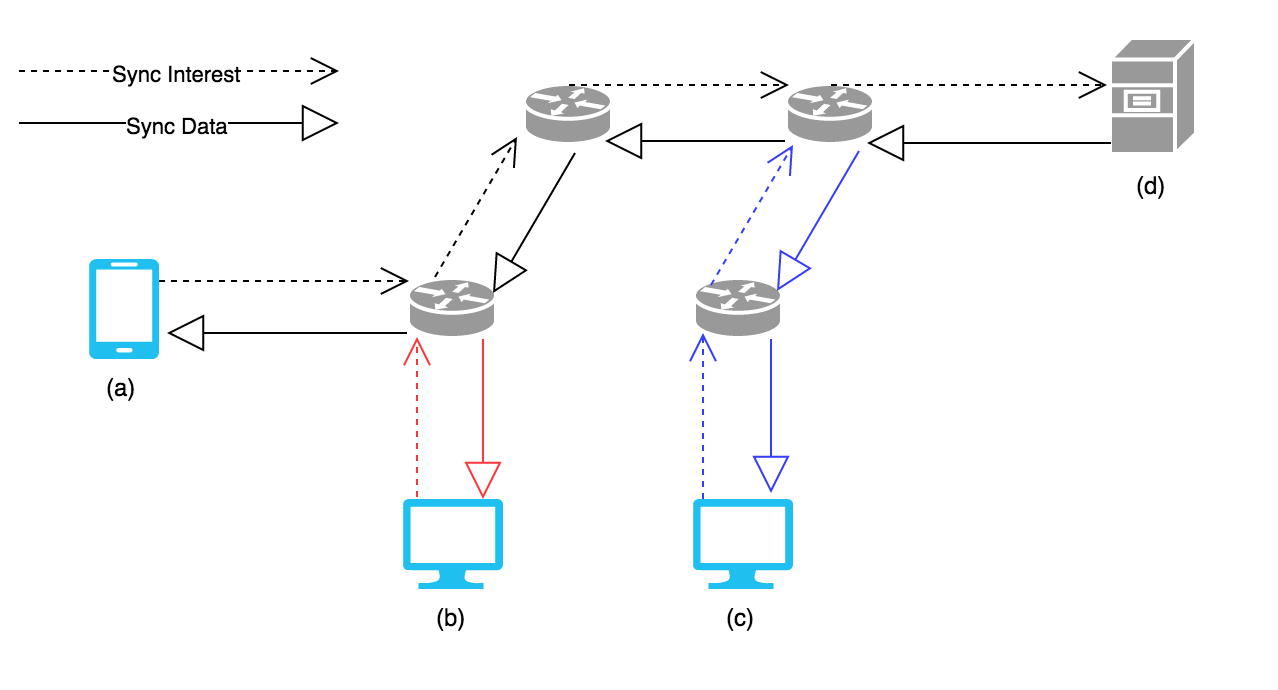
\includegraphics[width=1\textwidth]{ndn-sync.png}
  \caption{File Synchronization in NDN.}
  \label{fig:ndn-sync}
\end{figure}

There are some issues that could occur. 
\gls{DoS} on Sync Interest and Sync Data. 
If the \gls{FSM} is used to revoke public keys as suggested, an attacker who has found the compromised private key, can try to deny the distribution of the new list, i.e. the Sync Data, from the distributor. 
